\section{Objective function and problem design}\label{sec:design}
Let \(\mathcal X=[-4,4]^2\), \(a=(-2,0)\), \(b=(2,0)\), and
\(r_0=0.5\). We minimise
\begin{equation}
\label{eq:objective}
 f_c(x)=\min\!\left\{
  1+\lVert x-a\rVert_2^2,\,
  h_c(\lVert x-b\rVert_2)
 \right\},
 \qquad
 h_c(r)=r^2+c(r-r_0)_+^2,
 \quad c\geq0,
\end{equation}
where \(u_+=\max(0,u)\). The minima at \(a\) and \(b\) have values 1 and 0, respectively; we refer to their associated basins as A and B. Within the radius-\(r_0\) core around \(b\), the objective is \(f_c(x)=\lVert x-b\rVert_2^2\), with Hessian \(2I_2\), for every penalty. Increasing \(c\) leaves the local neighbourhood of the global minimum unchanged.

We define discovery as observing \(f_c(x)<1\), thereby improving on the best value achievable in A. Since the first term in \eqref{eq:objective} is at least 1, the discovery set is precisely the open disk around \(b\) with radius
\begin{equation}
\label{eq:radius}
 \rho_c=
 \frac{cr_0+\sqrt{1+c(1-r_0^2)}}{1+c},
 \qquad h_c(\rho_c)=1.
\end{equation}
At \(c=0,3,10,30\), these radii are approximately \(1.000,0.826,0.720,0.640\). Precision means observing \(f_c(x)<10^{-2}\), which always defines a disk of radius \(0.1\). Figure~\ref{fig:geometry} illustrates this construction.

\begin{figure}[!htb]
 \centering
 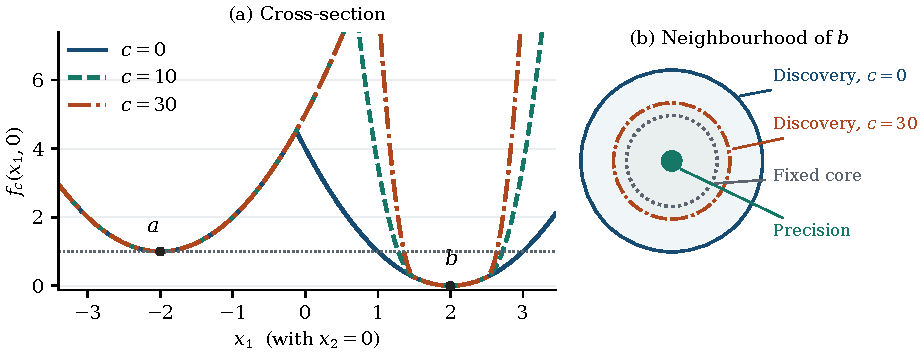
\includegraphics[width=.96\linewidth]{problem_geometry.pdf}
 \caption{Objective cross-section at \(x_2=0\) and target sets around \(b\). The discovery radius depends on \(c\). The fixed core and precision circle are unchanged and have radii \(0.5\) and \(0.1\), respectively.}
 \label{fig:geometry}
\end{figure}

Every main comparison uses \(T=50\) objective evaluations. In our experiments, unless otherwise stated, BO-EI uses four initial random evaluations, EI offset \(\xi=0\) and a GP noise parameter of \(10^{-10}\) for numerical stability. TuRBO-1 uses four initial design evaluations per start, batch size one and 50 GP training steps. CMA-ES uses a uniformly sampled initial mean on \([0,1]^2\), the default \texttt{pycma} population size, and initial step size \(\sigma_0=0.25\), corresponding to 2 units in the original coordinates. The implementation restarts if CMA-ES terminates before the budget is exhausted. Uniform random search draws independently from \(\mathcal X\).

Let \(F_t=\min_{1\leq i\leq t}f_c(x_i)\). Since \(f_c(b)=0\), \(F_t\) is the simple regret, ie. the difference between the found minimum and the true global minimum. We report empirical attainment of discovery, core entry and precision, corresponding to thresholds \(1\), \(0.25\) and \(10^{-2}\), together with terminal regret and first hitting times \cite{coco}. A missed target has hitting time \(+\infty\) by default. 





